\documentclass[11pt, a4paper]{article}

% --- Packages ---
\usepackage[utf8]{inputenc}
\usepackage{amsmath}
\usepackage{graphicx}
\usepackage{geometry}
\usepackage{float}
\usepackage{caption}

\geometry{margin=1in}

% --- Title Information ---
\title{{\bf MLDS HOMEWORK 1} \\
(TREES AND RANDOM FOREST)}
\author{Denis Nedić}
\date{\today}

\begin{document}

\maketitle
\vspace{-1cm} % Pulls the first section up slightly to save space

\section{Model Performance and Uncertainty}
To evaluate our models without having to train them many times over, we can look at the predictions as independent Bernoulli trials. We calculate the uncertainty using the Standard Error (SE) formula for a binomial proportion: $SE = \sqrt{p(1 - p)/N}$, where $p$ is the misclassification rate and $N$ is the number of samples in the dataset we are testing.

Table \ref{tab:results} summarizes the results for a single decision tree compared to a Random Forest with 100 trees.

\begin{table}[H]
    \centering
    \caption{Misclassification Rates: Single Tree vs. Random Forest}
    \label{tab:results}
    \begin{tabular}{l c c c c}
        \hline
        \textbf{Model} & \textbf{Train Error} & \textbf{Train SE} & \textbf{Test Error} & \textbf{Test SE} \\
        \hline
        Single Tree & 0.0000 & 0.0000 & 0.3167 & 0.0601 \\
        Random Forest & 0.0000 & 0.0000 & 0.2333 & 0.0546 \\
        \hline
    \end{tabular}
\end{table}

As we can see, the single tree completely memorized the training data (0.0000 error). However, it performed poorly on the test set with an error of 0.3167, which means it overfitted heavily. The Random Forest fixed this problem. By averaging the predictions from 100 different trees, the test misclassification rate dropped to 0.2333, showing that the ensemble generalizes much better to new data.
\vspace{-2mm}
\section{Effect of Forest Size on Misclassification}
To see how the size of the forest changes the performance, we plotted the misclassification rate against the number of trees ($n$).

\begin{figure}[H]
    \centering
    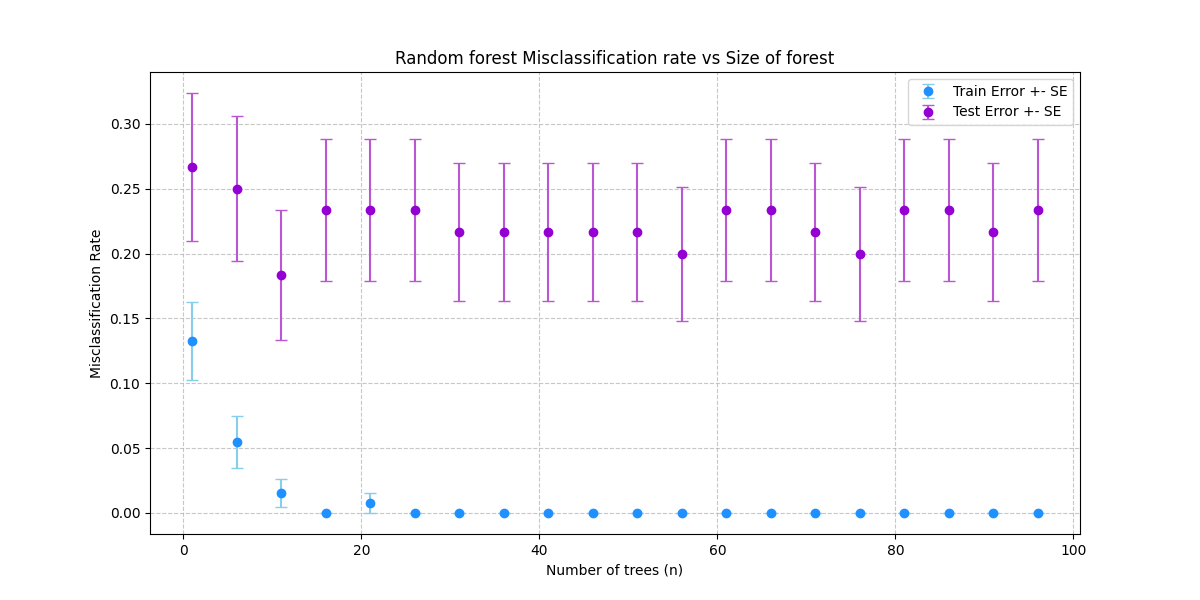
\includegraphics[width=0.75\textwidth]{miss.png}
    \caption{Misclassification rates ($\pm$ SE) for training and testing datasets across different forest sizes.}
    \label{fig:miss}
\end{figure}

In Figure \ref{fig:miss}, the training error (blue dots) quickly goes to zero. The test error (purple dots) starts very high when $n=1$, but it drops fast as we add the first few trees. After that, it flattens out when $n$ gets closer to 100. This shows a well-known property of Random Forests: adding more trees helps the model stabilize and does not make the overfitting worse.

\section{Variable Importance Analysis}
To find out which spectral features actually predict TKI resistance, we calculated the Out-of-Bag (OOB) permutation importance for our Random Forest. But decision trees sometimes pick features just because they have a high mathematical variance. To check if our signals are real, we compared them to a null model. For this null model, we completely shuffled the target labels to make the data random, trained 100 standard trees on it, and counted how many times each feature was used at the root.

\begin{figure}[H]
    \centering
    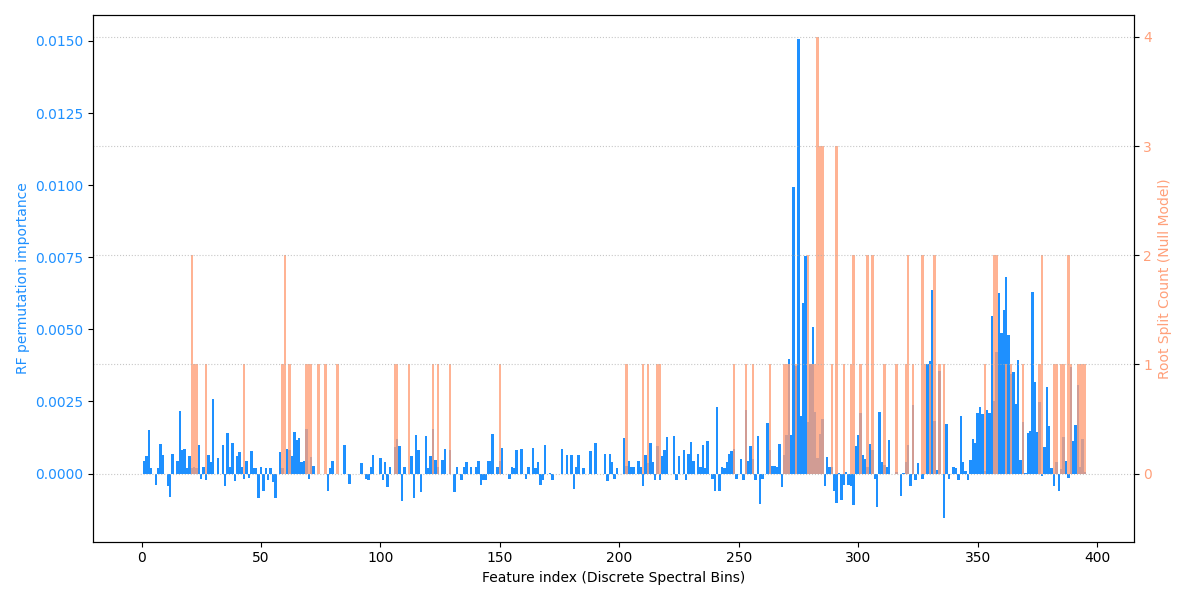
\includegraphics[width=0.85\textwidth]{import.png}
    \caption{OOB permutation importance (blue) vs. null model root split frequencies (salmon).}
    \label{fig:importance}
\end{figure}

Figure \ref{fig:importance} shows the clear difference between real signals and random noise. If we look very closely at the features between index 270 and 290, we can see something really interesting. There are big blue spikes of importance, but the salmon spikes from the random null model do not perfectly overlap with the highest blue peaks. Instead, the random noise pops up right next to them, exactly where the real importance is dropping. This tells us that the highest peaks in that 270–290 range are actually genuine signals, and our Random Forest was smart enough to separate them from the noisy features right next door. Furthermore, we also have a very clear, clean signal around features 350 to 370 where the null model is completely flat. Finally, the features that drop into negative importance almost perfectly match the flat parts of the null model, proving they are just useless background noise.

\end{document}